\section{Utterance Embeddings}\label{sec:utt2vec}
\roger{This section still contains some redundant parts and needs to be restructured.}
\david{I did a first attempt at fixing it, but it still needs some (small) updates}

\subsection{Word Embeddings}
Neural networks for distributional semantics has gained relevant importance in the past years since the publication of the first neural network word embedding models. One of the main reasons for that was the discovery that dense high-dimensional vector representations of words are able to capture semantic relations between words \newcite{mikolov2013efficient}.  Figure~\ref{fig:w2v_example} shows a typical example where simple vector addition and subtraction lead to analogies such as, the vector difference between \textit{woman} and \textit{man} is the same as between \textit{aunt} and \textit{uncle}.


\begin{figure}
\centering
\begin{minipage}{.4\textwidth}
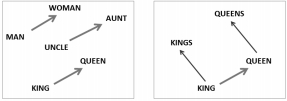
\includegraphics[width=1\textwidth]{img/w2v_example}
\caption{Word2vec semantic relations.}
\label{fig:w2v_example}
\end{minipage}
\end{figure}

In distributional semantic models, word embeddings are learned by predicting words within a context of other words. Based on the fact that similar words occur in similar contexts, these models are capable of successfully representing words in high-dimensional vectors \newcite{mikolov2013efficient}. 
%In order to get vector representations from utterances, we use an extension of the word embeddings neural network proposed by Mikolov\cite{mikolov2013efficient}. 

Originally, these networks had two main architectures, know as \emph{Continuous-bag-of-words} and \emph{Skip-gram}. In the first case, the networks were optimized to predict the next word given its context, while in the latter, the context is predicted given a certain word. Due to word co-occurrences, these models are able to effectively capture the meaning of the words. 
%The co-occurrence property present at the word level is no longer valid when handling phrases.

\subsection{Paragraph embeddings} 
The approach from \newcite{mikolov2013efficient} is no longer feasible on a sentence level, as the vocabulary of all observed sentences is larger \david{isn't it infinitely large? as we can construct a sentence of any lenght?} than the word-based vocabulary leading to sparse contexts. Therefore, a slightly different neural network approach for learning representations of sentences has been proposed by \shortcite{le2014distributed}, in which sentence vectors are learned from the words within the sentences. In this case, sentence embeddings are trained together with word embeddings. The latter are shared for the entire model.

In this case, two structures are maintained one for words, and one for sentence representations. The word structure is shared across all sentences, while the sentence structure is only valid for the current paragraph. The training task is the same as before: given a certain window, the model is optimized to predict the missing word. However this time, the context representation is constructed using the individual word vectors together with the paragraph vector. This training schema is called \emph{Paragraph Vector Distributed memory (PV-DM)}, and it is the one we use to train our model. Figure~\ref{fig:p2v_arq} shows the \emph{PV-DM} architecture.

This model makes it possible to map word sequences of any length to vectors of fixed dimensionality. Moreover, its unsupervised nature allows any unannotated corpus to be used for training.

%\david{as the paragraphs above might be the complicated part of our research we should spend some time getting this as clear and readable as possible}

%\roger{The part below should be merged with the part above.}

\begin{figure}
\centering
\begin{minipage}{.3\textwidth}
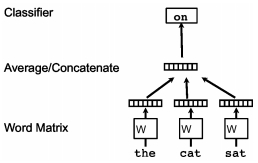
\includegraphics[width=1\textwidth]{img/par2vec_arq}
\caption{Paragraph vector PV-DM architecture.}
\label{fig:p2v_arq}
\end{minipage}
\end{figure}

Once the model is trained, it can be queried in order to get the vector representations for each previously seen sentence. It can also be used to \emph{infer} vector mappings of \emph{unseen} sentences. This second step will be crucial to get representations for utterances in our test dataset.

The approach presented by \newcite{le2014distributed} has two very nice advantages. Firstly it is completely unsupervised, and thus, we can use any amount of unannotated data that is available.

%\subsubsection*{Word2vec pretrained vectors} 
\david{i dont think we need this as a spererate subsubsection? but alternatively merge the previous and next paragraph talking about the advantages of the model}

Moreover we can use pretrained word embeddings. This can be summarized as follows: (a) No new words are added to the vocabulary; (b) Intersecting words adopt pretrained values ; (c) Non intersecting words are left alone. \david{maybe explain this a bit better/more in depth?}
For our experiments, we try different alternatives, training word and paragraph embeddings from scratch using several different dialog corpora as input, and also using freely available pretrained word embeddings\footnote{\url{https://code.google.com/p/word2vec/}}. In the next section we specify the different ways and corpora we used for learning utterance embeddings. \david{this ok?}